\subsection{Firebase}
\label{sec:firebase}

Firebase ist eine Plattform von Google, welche es Entwickler:innen ermöglicht, eine Vielzahl von Funktionen in ihre Applikationen zu integrieren. Diese Funktionen sind zum Beispiel Authentifizierung, Datenbanken, Cloud Messaging und Hosting. Die Plattform ist für kleine Projekte kostenlos und bietet eine kostenlose Testversion mit 1 GB Speicherplatz und 50.000 Anfragen pro Tag. Firebase vereinfacht das Entwickeln von Mobil- und Webapplikationen, da die Entwickler:innen sich nicht um die Infrastruktur kümmern müssen. Die Plattform ist in verschiedene Komponenten aufgeteilt, die einzeln oder zusammen verwendet werden können. Firebase verwendet ein \enquote{pay as you go} Modell bei dem Nutzer:innen pro Anfrage einen bestimmten Betrag bezahlen. Firebase ist Teil von Google Cloud Platform.

\begin{figure}[h]
  \centering
  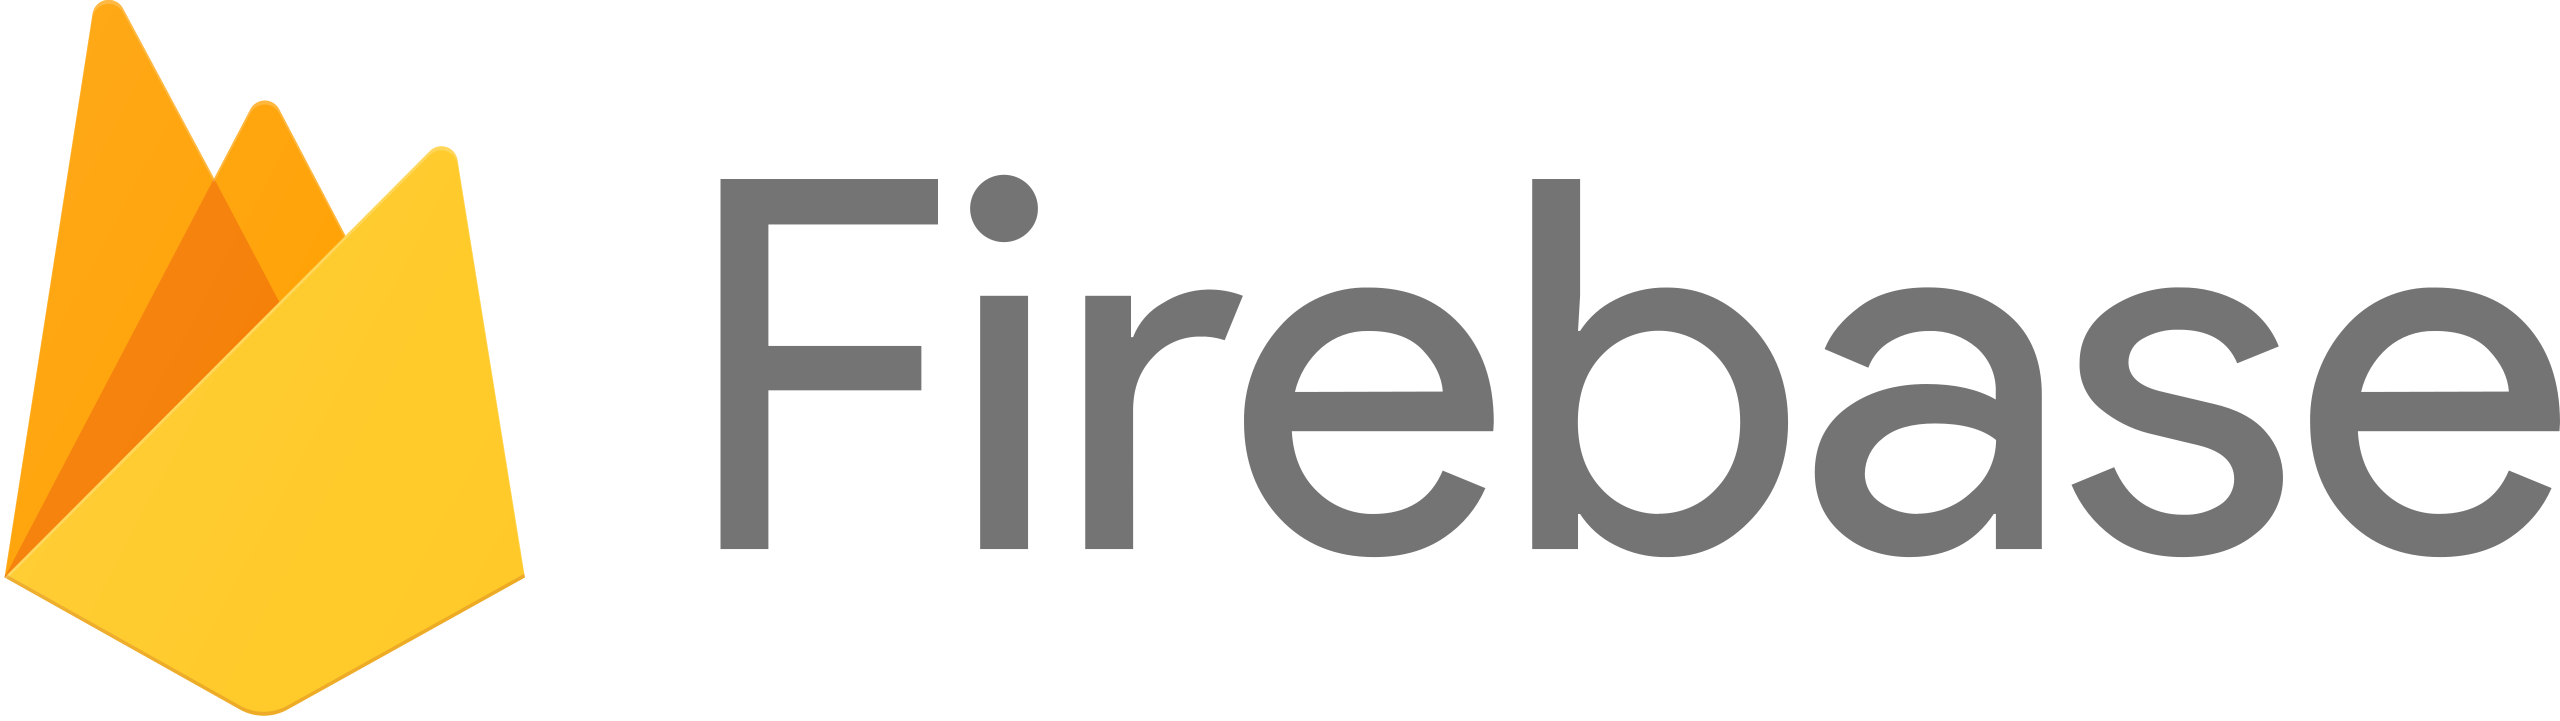
\includegraphics[width=0.5\textwidth]{images/firebase_logo}
  \caption{Firebase Logo \citev{firebase_logo}}
  \label{fig:firebase_logo}
\end{figure}

Um die Entwicklung weiter zu vereinfachen, bietet Google offizielle Firebase \acp{SDK} für viele gängige Programmiersprachen an. Diese \acp{SDK} bieten eine einfache \ac{API}, welche die Kommunikation mit der Plattform vereinfacht. Die \ac{API} ist sehr detailliert dokumentiert, weshalb es auch \acp{SDK} für andere Programmiersprachen gibt.

Firebase vereinfacht zwar die urprüngliche Entwicklung, jedoch gibt es das Problem von \enquote{Vendor Lock-in}. Dies bedeutet, dass die Entwickler:innen auf die Plattform von Firebase angewiesen sind, da diese sehr eng mit Applikationen integriert sind.
